\chapter{Cibles de fonctionnement}


\section{Axes d'amélioration}

    Les chapitres précédents --- analyse de l'existant et benchmarking -- permettent d'identifier quelques axes sur lesquels le système d'information de SPIE péche contre les bonnes pratiques et où des améliorations sont à prévoir.

    Nous allons donc citer dans ce document certains thèmes d'amélioration possibles à travers les axes suivant:

    \begin{enumerate}
        \item Identification de nouvelles technologies à forte valeur ajoutée~;
        \item Réorganisation des acteurs des processus métiers de SPIE pour suivre les ``best-practices'' dégagées~;
        \item Réorganisation de la logique des processus existants~;
    \end{enumerate}


    \subsection{Nouvelles technologies}

    L'intégration de nouvelles technologies peut permettre à SPIE de se démarquer de la concurrence en changeant de manière radicale la gestion de certaines opérations.

    Nous allons nous intéresser à certaines technologies que SPIE pourrait intégrer~:

        \subsubsection{Gestion de la Relation Client avec un CRM}

            Quand on s'intéresse à la cartographie générale du SI de SPIE, la première chose qu'on remarque est l'absence d'une gestion de la Relation Client en utilisant un outil dédié, de type CRM.

            Les outils CRM (\textit{Customer Relationship Management}, ou Gestion de la Relation Client) permettent une gestion optimale la Relation Client avec des outils de modélisation, de reporting et de prédiction.

            L'utilisation d'outils dédiés permet autant d'améliorer les processus de Relation Client que de prédire les attentes de clients et ainsi prévenir les échecs et mieux s'y préparer. Là où SPIE utilise actuellement plusieurs outils (\textit{Clarify}, \textit{ADV}, \textit{SUPRA}) aux infrastructures parfois séparées, l'utilisation d'un seul CRM simplifierai les processus de facturation, de suivi contrats et autres processus clients, et permettrait une meilleure intégration entre ces derniers.

            Les outils CRM permettent en outre de mener des campagnes de prospection, de suivre les opportunités commerciales et de fidéliser les clients.

            On peut citer à titre d'exemple \textit{Salesforce}, l'un des leaders du marché qui propose un CRM en mode \textit{SaaS}.

        \subsubsection{SI utilisable pendant les interventions (application mobile)}

            Les techniciens ne peuvent actuellement pas utiliser les applications SPIE pendant une intervention: ils ne disposent pas de tablettes fournies à ce but et les applications SPIE ne sont pas optimisés (ou même parfois utilisables) sur des terminaux mobiles.

            Fournir des tablettes aux techniciens et leur donner accès au système d'information de SPIE leur permettrait de proposer une meilleur service aux clients chez lesquels ils interviennent en ayant constamment sous les yeux les informations relatives à des interventions précédentes (par eux ou d'autres techniciens), et pouvant entrer au fur et à mesure des informations sur le déroulement de l'intervention afin d'assurer une meilleure réactivité et afin qu'aucune information ne soit oubliée (ce qui risque d'arriver si le technicien ne fait l'entrée de données qu'une fois l'intervention terminée).

            Il faut noter que les éditeurs d'ERPs, et plus généralement de logiciels modernes adoptent souvent aujourd'hui une politique de \textit{``Mobile first''} et proposent ainsi des outils accessibles aussi bien depuis ordinateur que depuis mobile et tablettes, sans sacrifier les fonctionnalités de l'ERP ou son ergonomie. SAP ByDesign s'adapte ainsi directement au terminal utilisé pour y accéder, et l'éditeur de CRM \textit{Salesforce} propose un \textit{framework} CRM adapté pour mobile, \textit{Salesforce1}, s'intégrant avec la totalité de sa ligne de produit.


        \subsubsection{Moteur de recommandation et de préventions des risques}

            SPIE peut valoriser ses années d'expérience dans le domaine de la maintenance en créant un moteur de recommandation exploitant toutes les données récoltées lors d'interventions passées afin de proposer aux techniciens des recommandations similaires à celle qu'ils souhaitent effectuer.

            De cette manière, l'expérience des techniciens SPIE sera réellement mutualisée et mise à profit~:

            \begin{itemize}
                \item Priorisation des points à vérifier pendant l'intervention, ce qui permet d'assurer des interventions rapides et efficaces~;
                \item Prévention d'erreurs commises lors d'interventions similaires~;
                \item Possibilité de contacter facilement un technicien étant intervenu dans un cas similaire afin de faire un partage d'information.
            \end{itemize}

            Les critères à privilégier pour recommander des livraisons sont nombreux. En voici quelque uns~:
            \begin{itemize}
                \item Client visé par l'intervention~;
                \item Matériel utilisé~;
                \item Zone géographique~;
                \item ``Symptomes'' de panne~;
                \item ...
            \end{itemize}

    % TODO : donner + de nouvelles technologies et notamment parler de ça :
    %
    % * Affecter un (ou des) techniciens à chaque client. Le technicien connaîtra déjà l'infrastructure du client à chaque intervention ce qui devrait accélérer les choses et donner un meilleur processus


\section{Les attentes client}

	Les clients ont certaines attentes lorsqu'ils signent un contrat (qui varient selon le client). Ci dessous nous allons lister les plus importantes d'entre elles qui peuvent apparaître.

\begin{itemize}
	\item une certaine proximité (couvrir le territoire)~;
	\item un support technologique~;
	\item de l'innovation~;
	\item de l'expertise~;

	\item assurer la gestion contractuelle et le reporting~;
	\item gérer les interventions (intervention forfaitaire : préventive et curative standard ; intervention en bon de commande : curative exceptionnelle, amélioration installations, traitement obsolescence...)~;
	\item une identification des risques techniques, financiers et organisationnels~;
	\item un compte rendu de l'état des lieux initial (pour les soldes d'écart si des travaux en plus sont nécessaires~;

	\item une améliorer le cadre de vie~;
	\item un respecter l'environnement~;

	\item un accompagnement dans la conception, la réalisation, l'exploitation et la maintenance~; d'installations plus économes en énergie et plus respectueuse de l'environnement~;
	\item un suivi des spécifications du client~;
	\item un suivi des avancements pour le client~;
	\item une construction et validation des processus avec le client~;
	\item une revue périodique du contrat pour les décisions à renouveler ou non, et la prise en compte de réclamations du client~;
	\item des preuves du respect des engagements (bonne mise en œuvre, et adaptation au besoin).
\end{itemize}


\section{Les nouvelles règles de gestion}
    Dans cette partie, nous allons proposer certaines règles standard qui pourront aider à réduire les dysfonctionnements dans la gestion des contrats de maintenance.


\section{Processus Retour d'expérience}

\begin{figure}[h!]
	\centering
	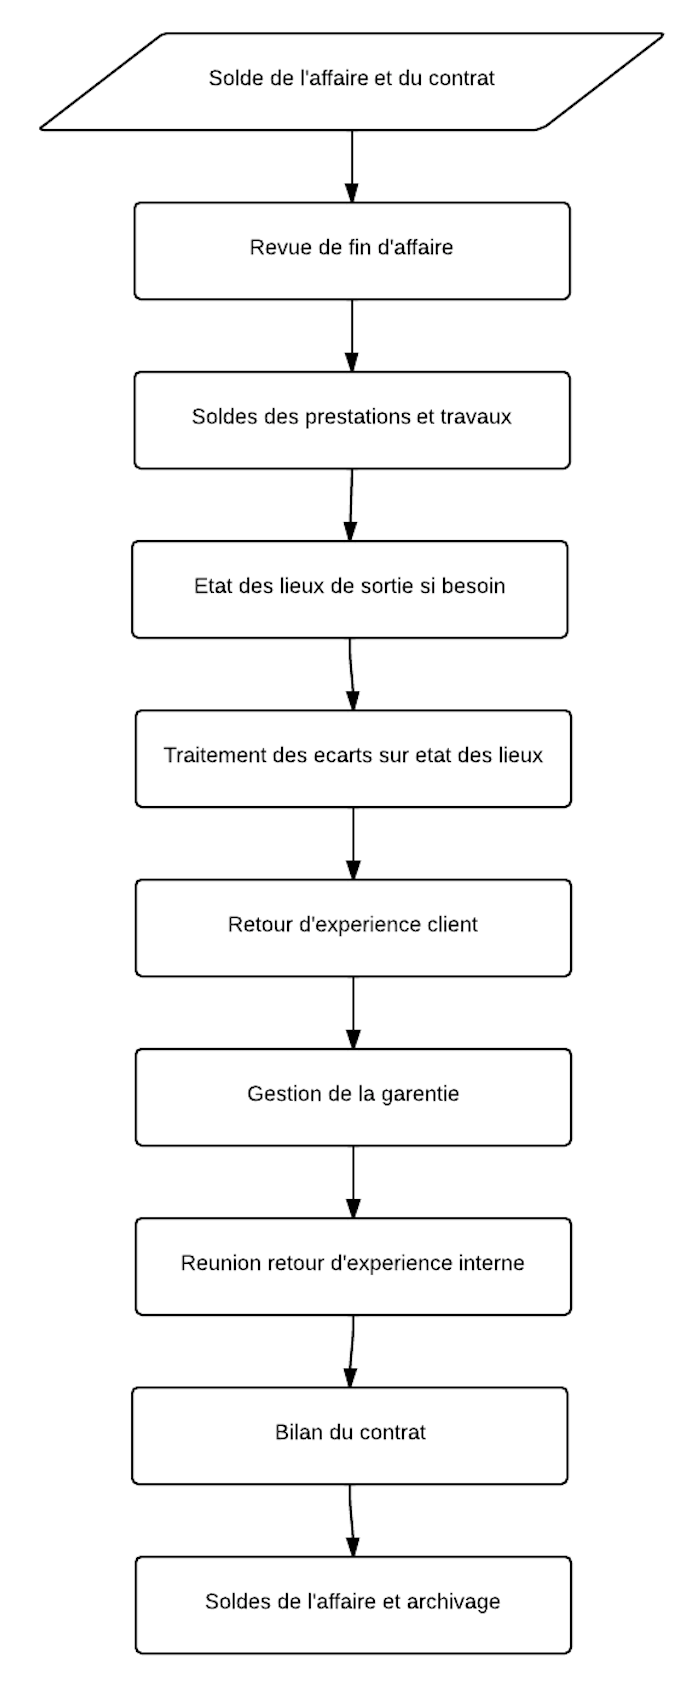
\includegraphics[width=0.45\linewidth]{images/processus_retour_experience.png}
	\caption{Processus de retour d’expérience}
	\label{fig:processusRetourExperience}
\end{figure}

Ainsi l'ajout du processus \textit{retour d'\'exp\'erience client} dans le sous-processus \textit{solde
de l'affaire et du contrat} r\'epond aux exigences de SPIE Sud Est suivante~:

\begin{itemize}
    \item Base de connaissance m\'etier type de contrat~;
    \item Identification des risques techniques/financiers/organisationnels.
\end{itemize}

